Given a log $(E_L, T_L, C_L)$ exhibiting an invariant violation,
our goal is to identify its MCS. Achieving this goal involves two tasks:
searching for subsequences of $E_L$, and searching for replay timings for each of those
subsequences.

\subsection{Searching for Subsequences}
\label{subsec:delta_debugging}

Checking random subsequences of $E_L$ would be one viable but inefficient
approach to achieving our first task. We can do better by leveraging a
divide-and-conquer search technique from the software engineering community:
the delta
debugging algorithm~\cite{Zeller:1999:YMP:318773.318946} provides a provably
correct\footnote{We do not have room to delve into the details of delta-debugging, but a few comments might be helpful. The original formulation of delta debugging\cite{Zeller:1999:YMP:318773.318946}
made three
assumptions about inputs: monotonicity, unambiguity, and consistency.
Violating the first two only leads to slightly inflated MCSes. We ensure that
intermediate subsequences are consistent (\ie~do not result in unresolved
outcomes) by checking for validity based on domain knowledge of the semantics
of network events. For example, we ensure that no recovery events occur
without a preceding failure event. Zeller wrote a follow-on
paper~\cite{Zeller:2002:SIF:506201.506206} that removes the need for this assumption,
but incurs an additional factor of $N$ in complexity in doing so.}
means to isolating fault-inducing inputs. In our case, we use delta
debugging to iteratively select subsequences of $E_L$, replay each
subsequence with
some timing $T$, and check whether the bug persists. If the bug persists,
delta debugging ignores the
other inputs, and proceeds with the search for an MCS within this subsequence.
In what follows, we use the term {\em delta-debugging} to refer to our algorithm for finding relevant subsequences.

\subsection{Searching for Timings}
\label{subsec:algorithm}

Simply exploring subsequences of $E_L$ does not suffice to find
minimal causal sequences: the
timing of those subsequences during replays is crucial for reliably
reproducing the
invariant violation. The most natural approach would be to maintain the original
timings, \ie~if we
define $t_i$ as the timestamp of the $i^{th}$ input from the original run and $t'_i$ as the
replay clock value when it injects that same input
(which may or may not be the $i$'th input in the subsequence), then we might just set $t'_i = t_i$
\eat{
\begin{align*}
t'_0 = t_0 \\
t'_i = t'_{i-1} + |t_{i} - t_{i-1}|
\end{align*}
}
Unfortunately, this approach does not work in practice because it can violate
causal dependencies. The crucial point here is that when we replay only a
subsequence of the original inputs, the reaction of the control software
can change, such that it behaves differently or takes a different amount of
time to respond to the remaining inputs events.
Simply maintaining relative timings might therefore
result in injecting the remaining inputs too early or too late.

Formally, to reliably reproduce the original invariant violation
we need to
inject an external input $e$ only after all other
events (both external and internal) that precede it in the
happens-before~\cite{Lamport:1978:TCO:359545.359563}
relation ($\{i \mid i \rightarrow e\}$) from the original execution have
occurred~\cite{tel2000introduction}. Internal events might include messages
sent between the controllers and switches, or state transitions within a single
controller. We can obtain the
happens-before relation in our logs by having our simulator
(to be described later) interpose on all message channels and
log a message only after all other logged messages have been delivered.

\subsection{Preserving Causality}

Unfortunately, it is non-trivial to reason about causal dependencies when transforming the original log
(which reproduces the violation) to a subsequence of external events
(which may or may not reproduce that violation).
To make progress we process the happens-before
relations reflected in the original log,
and draw inferences about
the remaining causal dependencies in the subsequence.
This involves three issues: coping with syntactic differences in internal
events across runs, handling internal events from the original
execution that may not occur after pruning, and dealing with new internal events that were not
observed at all in the original execution.

\eat{
\colin{Somewhat redundant. Maybe wait until use cases.}
While the inputs and original internal events are given to us,
we become aware of new internal events throughout replay by
(i) monitoring
control message receipts between controllers and switches,
and (ii) interposing on the controllers' logging library and notifying the
simulator whenever the control software executes a log statement (which serve to mark relevant state
transitions). Note that to achieve truly deterministic
replay, these log statements would need to
be highly granular, capturing information such as thread scheduling decisions;
we show in \S\ref{subsec:case_studies}
however that pre-existing, course granular log statements are often sufficient to
successfully reproduce bugs.
}
%\footnote{We discuss this problem further in
%\S\ref{subsec:domain_knowledge}.}
%Note that the developer must provide enough logging statements
%so that relevant internal state changes are captured and visible to our
%tool.

{\bf Functional Equivalence: }The first issue is that internal events may differ syntactically (\eg~sequence numbers
of control packets may all differ) when replaying a subsequence of the original log.
We observe that many internal events are {\em functionally
equivalent}, in the sense that they
have the same effect on the state of the system with respect to triggering the
invariant violation (despite syntactic differences). For example, flow
modification messages may cause switches to make the same change to their forwarding behavior
even if the transaction identifier of the messages differ.

We leverage this observation by defining
domain-specific masks over semantically extraneous fields of
internal events.\footnote{One consequence
of applying masks is that bugs involving masked fields are outside the purview of
our approach.} We show four examples of masked values
in Table~\ref{tab:fingerprints}. We consider an internal event $i'$ observed in the subsequence log
equivalent (in the sense of inheriting all of its happens-before relations) to an internal event $i$ from the original log iff all unmasked
fields have the same value
and $i$ occurs between $i'$'s preceding and succeeding inputs in the
happens-before relation.

\eat{
\begin{figure}[t]
    %\hspace{-10pt}
    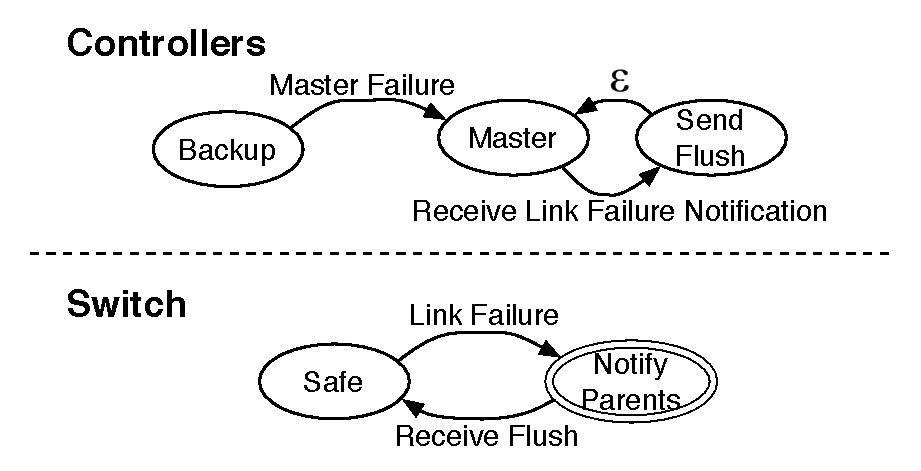
\includegraphics[width=3.25in]{../diagrams/state_machines/controller_switch.pdf}
    \caption[]{\label{fig:state_machines} Simplified state machines for the switch and
    controllers in the example Floodlight bug. Double outlined states
    represent presence of the blackhole.}
\end{figure}
}

\begin{table}
\centering
\begin{tabular}{|l|l|}
\hline
Internal message & Masked values \\
\hline
OpenFlow headers & transaction id\\
OpenFlow FLOW\_MODs & cookie, buffer id \\
Log statements & varargs parameters to printf \\
\hline
\end{tabular}
\caption{Example internal messages and their masked values. The masks serve to
define equivalence classes.}
\label{tab:fingerprints}
\end{table}

{\bf Handling Absent Internal Events:}
\eat{Given an equivalence relation over internal events, $replay$
is responsible for maintaining equivalent happens-before constraints from the
original execution.
But syntactic differences are not the
only possible change induced by pruning: internal events
may also cease to appear.


The structure of the control
software's state machine (which we do not assume to know) determines whether
internal events disappear. Consider the simplified state machines for the switch and
controllers from the Floodlight case shown in
Figure~\ref{fig:state_machines}. If we prune the link failure input, the
master will never receive a link failure notification and
transition to and from `Send Flush'.
}
Some internal events from the original log, and which causally ``happen before'' some external event,
may be absent when replaying a subsequence of that log.
We therefore wait for expected equivalent internal events, but time out and proceed
if they do not occur within a certain time \textepsilon.
\eat{In most cases this heuristic successfully reproduces the original invariant
violation, assuming \textepsilon~is larger than variations in execution speeds
between internal events. If the value of \textepsilon~is too large, however, we may end up
waiting too long for the happens-before predecessors of an input $e_i$ such that a
successor of $e_i$ occurs before we have injected $e_i$,
thereby violating causality.}
If the event scheduling algorithm detects that it has waited too long (such
that a happens-before successor has occurred before a predecessor), it
replays the log from the beginning up until the immediately prior input, this time
knowing exactly which internal events in the current input interval are
and are not going to occur before injecting the next input. We show the overall event scheduling algorithm
in Figure~\ref{fig:peek}.

\begin{figure}
  \begin{pseudocode}[framebox]{CausalInference}{events}
    \PROCEDURE{Replay}{subsequence}
    \FOR e\textsubscript{i}\ in\ subsequence \\
    \BEGIN
    \IF e\textsubscript{i}\ is\ an\ internal\ event \\
    \AND e\textsubscript{i}\ is\ not\ marked\ absent:
    \THEN
    \BEGIN
      \Delta \GETS |e\textsubscript{i}.time - e\textsubscript{i-1}.time| + \epsilon \\
      wait\ up\ to\ \Delta\ seconds\ for\ e\textsubscript{i} \\
      \IF e\textsubscript{i}\ did\ not\ occur:
      \THEN mark\ e\textsubscript{i}\ as\ absent
    \END
    \ELSEIF e\textsubscript{i}\ is\ an\ input:
    \THEN
    \BEGIN
      \IF a\ successor\ of\ e\textsubscript{i}\ occurred: \\
      \INLINECOMMENT{waited too long}
      \THEN
        \RETURN{\CALL{Replay}{subsequence}}
      \ELSE
        inject\ e\textsubscript{i}
      \END
    \END
    \ENDPROCEDURE
  \end{pseudocode}
  \caption{{\tt Replay} is responsible for replaying subsequences of events
  chosen by delta debugging and determining
  if the bug reappears. \colin{Fix framebox width}}
    \label{fig:peek}
\end{figure}

%\begin{figure}
%\begin{boxedminipage}{\linewidth}
%\begin{Verbatim}[commandchars=\\\{\}]
%subsequence = [e\textsubscript{1}, e\textsubscript{2}, ..., e\textsubscript{j}]
%// e\textsubscript{1} is always an input
%
%function replay(subsequence):
%  bootstrap the simulation
%  for e\textsubscript{i} in subsequence:
%    if e\textsubscript{i} is an internal event and
%          e\textsubscript{i} is not marked absent:
%      \textDelta = |e\textsubscript{i}.time - e\textsubscript{i-1}.time| + \textepsilon
%      wait up to \textDelta seconds for e\textsubscript{i}
%      if e\textsubscript{i} did not occur:
%        mark e\textsubscript{i} absent
%    else if e\textsubscript{i} is an input:
%      if a successor of e\textsubscript{i} occurred:
%        // waited too long
%        return replay(subsequence)
%      else:
%        inject e\textsubscript{i}
%\end{Verbatim}
%\end{boxedminipage}
%\end{figure}

{\bf Handling New Internal Events:}
The last possible change induced by input pruning is the occurrence of new
internal events that were not observed in the original log.
New events ultimately leave open multiple possibilities for where
we should inject the next input. Consider the following case:
if $i_2$ and $i_3$ are internal events observed
during replay that are both in the same equivalence class as a single event $i_1$ from the
original run, we could inject the next input after $i_2$ or after $i_3$.

% TODO: figure this figure out
%\begin{wrapfigure}{c}{1.3\linewidth}
%  \centering
%  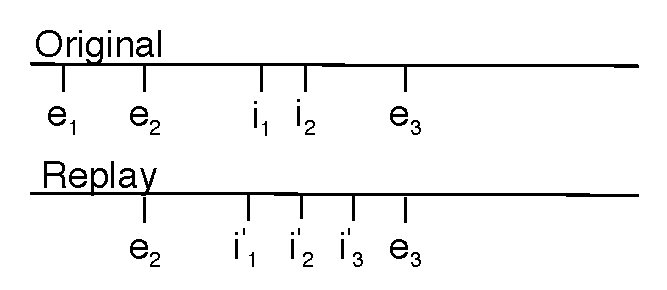
\includegraphics[width=\linewidth,height=0.8in]{../diagrams/state_machines/event_sequence.pdf}
%\end{wrapfigure}

\eat{In the general case it is always possible to construct two state machines that lead
to differing outcomes: one that only leads to the invariant violation when
we inject the next input
before a new internal event, and one that only leads to the
invariant violation when we inject the next input after a new internal
event. In other words, to be guaranteed to traverse any existing suffix that leads
to the invariant violation, it is necessary to recursively branch, trying both
possibilities for every new internal event. This implies an exponential number of
possibilities to be explored in the worst case.}

Exponential search over these possibilities is not a practical option. Our heuristic when waiting for expected internal
events is to proceed normally if there are intermediate new internal events,
always injecting the next input when its last expected predecessor
either occurs or times out. This ensures that we always find suffixes that
contain only a subset of the (equivalent) original internal events, but leaves open the
possibility of finding divergent suffixes that still lead to the invariant
violation.
%This is reasonable because not even branching on new
%internal events is guaranteed to find the globally shortest fault-inducing input
%sequence:
%there may be other unknown
%paths through the state machine leading to the invariant violation that are
%completely disjoint from the original execution.

\eat{
Luckily, crucially ambiguous new internal events are not problematic for the
control software we evaluated, as we show in \S\ref{sec:casestudies}.
We conjecture that ambiguous new internal events are
rare because SDN software is a control plane system,
and is designed to quiesce quickly (\ie~take a small number of internal
transitions after any input event, and stop at highly connected vertices).
Concretely, SDN programs are often structured as (mostly independent) event
handlers, meaning that pruning input events simply triggers a subset of the original
event handlers.
\eat{
As an illustration, consider the state machines
in Figure~\ref{fig:state_machines}:
the controllers quickly converge to a single state (either ``Master'' or
``Backup''), as do the switches (``Safe'').
}
}

In the next section we describe some
of the practical challenges we have overcome to realize our approach.
In our initial experiments we have found that applying delta debugging to explore
subsequences of $E_L$ and striving to maintain a single timing $T$ that maintains
causal dependencies reliably finds small MCSes.
